\documentclass[1p]{elsarticle_modified}
%\bibliographystyle{elsarticle-num}

%\usepackage[colorlinks]{hyperref}
%\usepackage{abbrmath_seonhwa} %\Abb, \Ascr, \Acal ,\Abf, \Afrak
\usepackage{amsfonts}
\usepackage{amssymb}
\usepackage{amsmath}
\usepackage{amsthm}
\usepackage{scalefnt}
\usepackage{amsbsy}
\usepackage{kotex}
\usepackage{caption}
\usepackage{subfig}
\usepackage{color}
\usepackage{graphicx}
\usepackage{xcolor} %% white, black, red, green, blue, cyan, magenta, yellow
\usepackage{float}
\usepackage{setspace}
\usepackage{hyperref}

\usepackage{tikz}
\usetikzlibrary{arrows}

\usepackage{multirow}
\usepackage{array} % fixed length table
\usepackage{hhline}

%%%%%%%%%%%%%%%%%%%%%
\makeatletter
\renewcommand*\env@matrix[1][\arraystretch]{%
	\edef\arraystretch{#1}%
	\hskip -\arraycolsep
	\let\@ifnextchar\new@ifnextchar
	\array{*\c@MaxMatrixCols c}}
\makeatother %https://tex.stackexchange.com/questions/14071/how-can-i-increase-the-line-spacing-in-a-matrix
%%%%%%%%%%%%%%%

\usepackage[normalem]{ulem}

\newcommand{\msout}[1]{\ifmmode\text{\sout{\ensuremath{#1}}}\else\sout{#1}\fi}
%SOURCE: \msout is \stkout macro in https://tex.stackexchange.com/questions/20609/strikeout-in-math-mode

\newcommand{\cancel}[1]{
	\ifmmode
	{\color{red}\msout{#1}}
	\else
	{\color{red}\sout{#1}}
	\fi
}

\newcommand{\add}[1]{
	{\color{blue}\uwave{#1}}
}

\newcommand{\replace}[2]{
	\ifmmode
	{\color{red}\msout{#1}}{\color{blue}\uwave{#2}}
	\else
	{\color{red}\sout{#1}}{\color{blue}\uwave{#2}}
	\fi
}

\newcommand{\Sol}{\mathcal{S}} %segment
\newcommand{\D}{D} %diagram
\newcommand{\A}{\mathcal{A}} %arc


%%%%%%%%%%%%%%%%%%%%%%%%%%%%%5 test

\def\sl{\operatorname{\textup{SL}}(2,\Cbb)}
\def\psl{\operatorname{\textup{PSL}}(2,\Cbb)}
\def\quan{\mkern 1mu \triangleright \mkern 1mu}

\theoremstyle{definition}
\newtheorem{thm}{Theorem}[section]
\newtheorem{prop}[thm]{Proposition}
\newtheorem{lem}[thm]{Lemma}
\newtheorem{ques}[thm]{Question}
\newtheorem{cor}[thm]{Corollary}
\newtheorem{defn}[thm]{Definition}
\newtheorem{exam}[thm]{Example}
\newtheorem{rmk}[thm]{Remark}
\newtheorem{alg}[thm]{Algorithm}

\newcommand{\I}{\sqrt{-1}}
\begin{document}

%\begin{frontmatter}
%
%\title{Boundary parabolic representations of knots up to 8 crossings}
%
%%% Group authors per affiliation:
%\author{Yunhi Cho} 
%\address{Department of Mathematics, University of Seoul, Seoul, Korea}
%\ead{yhcho@uos.ac.kr}
%
%
%\author{Seonhwa Kim} %\fnref{s_kim}}
%\address{Center for Geometry and Physics, Institute for Basic Science, Pohang, 37673, Korea}
%\ead{ryeona17@ibs.re.kr}
%
%\author{Hyuk Kim}
%\address{Department of Mathematical Sciences, Seoul National University, Seoul 08826, Korea}
%\ead{hyukkim@snu.ac.kr}
%
%\author{Seokbeom Yoon}
%\address{Department of Mathematical Sciences, Seoul National University, Seoul, 08826,  Korea}
%\ead{sbyoon15@snu.ac.kr}
%
%\begin{abstract}
%We find all boundary parabolic representation of knots up to 8 crossings.
%
%\end{abstract}
%\begin{keyword}
%    \MSC[2010] 57M25 
%\end{keyword}
%
%\end{frontmatter}

%\linenumbers
%\tableofcontents
%
\newcommand\colored[1]{\textcolor{white}{\rule[-0.35ex]{0.8em}{1.4ex}}\kern-0.8em\color{red} #1}%
%\newcommand\colored[1]{\textcolor{white}{ #1}\kern-2.17ex	\textcolor{white}{ #1}\kern-1.81ex	\textcolor{white}{ #1}\kern-2.15ex\color{red}#1	}

{\Large $\underline{11a_{1}~(K11a_{1})}$}

\setlength{\tabcolsep}{10pt}
\renewcommand{\arraystretch}{1.6}
\vspace{1cm}\begin{tabular}{m{100pt}>{\centering\arraybackslash}m{274pt}}
\multirow{5}{120pt}{
	\centering
	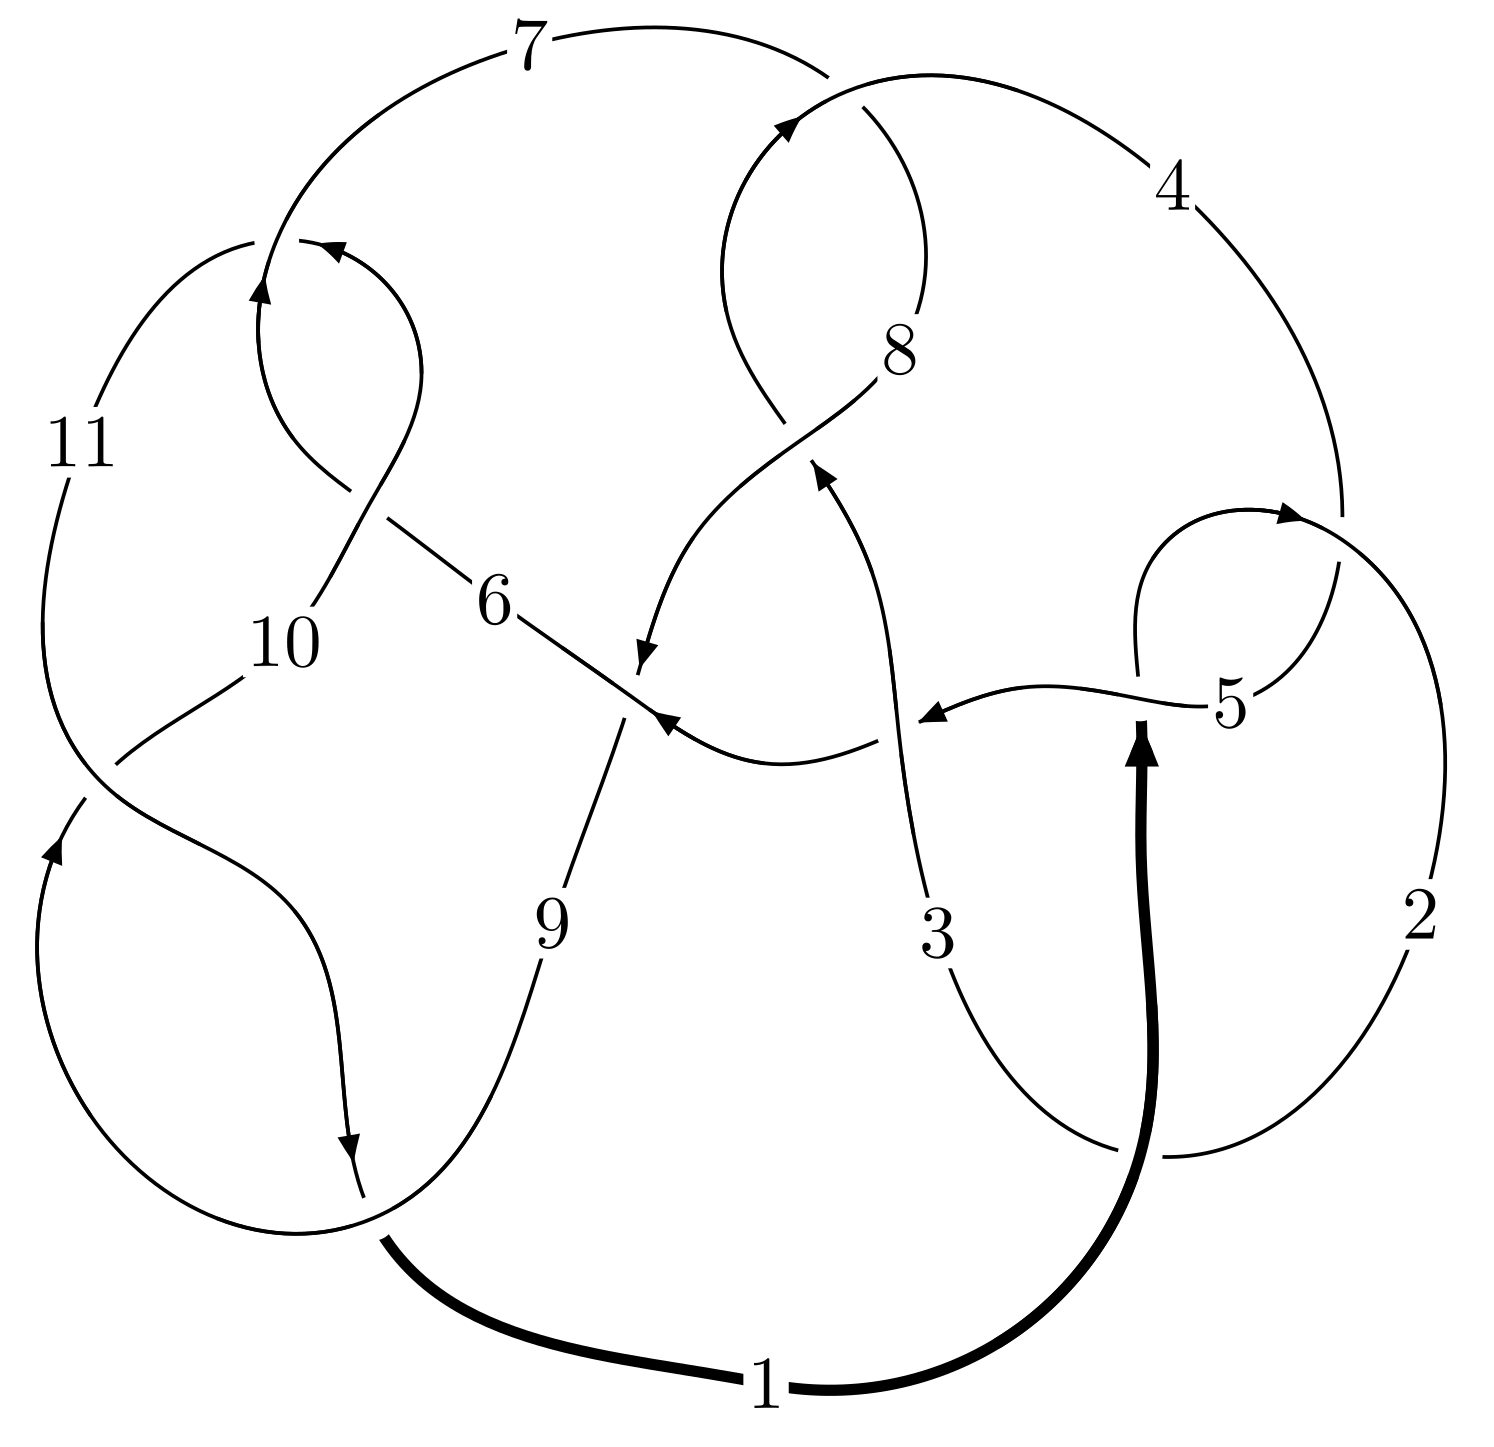
\includegraphics[width=112pt]{../../../GIT/diagram.site/Diagrams/png/250_11a_1.png}\\
\ \ \ A knot diagram\footnotemark}&
\allowdisplaybreaks
\textbf{Linearized knot diagam} \\
\cline{2-2}
 &
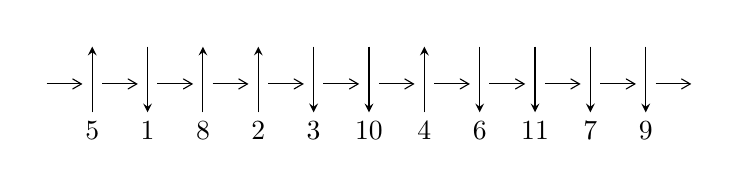
\begin{tikzpicture}[x=20pt, y=17pt]
	% nodes
	\node (C0) at (0, 0) {};
	\node (C1) at (1, 0) {};
	\node (C1U) at (1, +1) {};
	\node (C1D) at (1, -1) {5};

	\node (C2) at (2, 0) {};
	\node (C2U) at (2, +1) {};
	\node (C2D) at (2, -1) {1};

	\node (C3) at (3, 0) {};
	\node (C3U) at (3, +1) {};
	\node (C3D) at (3, -1) {8};

	\node (C4) at (4, 0) {};
	\node (C4U) at (4, +1) {};
	\node (C4D) at (4, -1) {2};

	\node (C5) at (5, 0) {};
	\node (C5U) at (5, +1) {};
	\node (C5D) at (5, -1) {3};

	\node (C6) at (6, 0) {};
	\node (C6U) at (6, +1) {};
	\node (C6D) at (6, -1) {10};

	\node (C7) at (7, 0) {};
	\node (C7U) at (7, +1) {};
	\node (C7D) at (7, -1) {4};

	\node (C8) at (8, 0) {};
	\node (C8U) at (8, +1) {};
	\node (C8D) at (8, -1) {6};

	\node (C9) at (9, 0) {};
	\node (C9U) at (9, +1) {};
	\node (C9D) at (9, -1) {11};

	\node (C10) at (10, 0) {};
	\node (C10U) at (10, +1) {};
	\node (C10D) at (10, -1) {7};

	\node (C11) at (11, 0) {};
	\node (C11U) at (11, +1) {};
	\node (C11D) at (11, -1) {9};
	\node (C12) at (12, 0) {};

	% arrows
	\draw[->,>={angle 60}]
	(C0) edge (C1) (C1) edge (C2) (C2) edge (C3) (C3) edge (C4) (C4) edge (C5) (C5) edge (C6) (C6) edge (C7) (C7) edge (C8) (C8) edge (C9) (C9) edge (C10) (C10) edge (C11) (C11) edge (C12) ;	\draw[->,>=stealth]
	(C1D) edge (C1U) (C2U) edge (C2D) (C3D) edge (C3U) (C4D) edge (C4U) (C5U) edge (C5D) (C6U) edge (C6D) (C7D) edge (C7U) (C8U) edge (C8D) (C9U) edge (C9D) (C10U) edge (C10D) (C11U) edge (C11D) ;
	\end{tikzpicture} \\
\hhline{~~} \\& 
\textbf{Solving Sequence} \\ \cline{2-2} 
 &
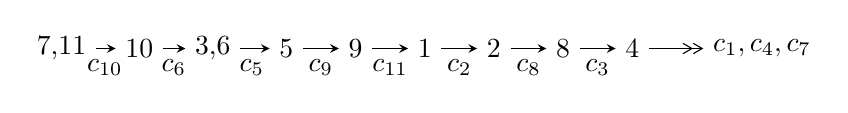
\begin{tikzpicture}[x=25pt, y=7pt]
	% node
	\node (A0) at (-1/8, 0) {7,11};
	\node (A1) at (1, 0) {10};
	\node (A2) at (33/16, 0) {3,6};
	\node (A3) at (25/8, 0) {5};
	\node (A4) at (33/8, 0) {9};
	\node (A5) at (41/8, 0) {1};
	\node (A6) at (49/8, 0) {2};
	\node (A7) at (57/8, 0) {8};
	\node (A8) at (65/8, 0) {4};
	\node (C1) at (1/2, -1) {$c_{10}$};
	\node (C2) at (3/2, -1) {$c_{6}$};
	\node (C3) at (21/8, -1) {$c_{5}$};
	\node (C4) at (29/8, -1) {$c_{9}$};
	\node (C5) at (37/8, -1) {$c_{11}$};
	\node (C6) at (45/8, -1) {$c_{2}$};
	\node (C7) at (53/8, -1) {$c_{8}$};
	\node (C8) at (61/8, -1) {$c_{3}$};
	\node (A9) at (10, 0) {$c_{1},c_{4},c_{7}$};

	% edge
	\draw[->,>=stealth]	
	(A0) edge (A1) (A1) edge (A2) (A2) edge (A3) (A3) edge (A4) (A4) edge (A5) (A5) edge (A6) (A6) edge (A7) (A7) edge (A8) ;
	\draw[->>,>={angle 60}]	
	(A8) edge (A9);
\end{tikzpicture} \\ 

\end{tabular} \\

\footnotetext{
The image of knot diagram is generated by the software ``\textbf{Draw programme}" developed by Andrew Bartholomew(\url{http://www.layer8.co.uk/maths/draw/index.htm\#Running-draw}), where we modified some parts for our purpose(\url{https://github.com/CATsTAILs/LinksPainter}).
}\phantom \\ \newline 
\centering \textbf{Ideals for irreducible components\footnotemark of $X_{\text{par}}$} 
 
\begin{align*}
I^u_{1}&=\langle 
4 u^{68}+5 u^{67}+\cdots+2 b+3 u,\;4 u^{68}+8 u^{67}+\cdots+a+2,\;u^{69}+3 u^{68}+\cdots+2 u+1\rangle \\
I^u_{2}&=\langle 
- u^2 b+b^2+b u- u+1,\;a,\;u^3- u^2+1\rangle \\
\\
\end{align*}
\raggedright * 2 irreducible components of $\dim_{\mathbb{C}}=0$, with total 75 representations.\\
\footnotetext{All coefficients of polynomials are rational numbers. But the coefficients are sometimes approximated in decimal forms when there is not enough margin.}
\newpage
\renewcommand{\arraystretch}{1}
\centering \section*{I. $I^u_{1}= \langle 4 u^{68}+5 u^{67}+\cdots+2 b+3 u,\;4 u^{68}+8 u^{67}+\cdots+a+2,\;u^{69}+3 u^{68}+\cdots+2 u+1 \rangle$}
\flushleft \textbf{(i) Arc colorings}\\
\begin{tabular}{m{7pt} m{180pt} m{7pt} m{180pt} }
\flushright $a_{7}=$&$\begin{pmatrix}0\\u\end{pmatrix}$ \\
\flushright $a_{11}=$&$\begin{pmatrix}1\\0\end{pmatrix}$ \\
\flushright $a_{10}=$&$\begin{pmatrix}1\\- u^2\end{pmatrix}$ \\
\flushright $a_{3}=$&$\begin{pmatrix}-4 u^{68}-8 u^{67}+\cdots-6 u-2\\-2 u^{68}-\frac{5}{2} u^{67}+\cdots-\frac{3}{2} u^3-\frac{3}{2} u\end{pmatrix}$ \\
\flushright $a_{6}=$&$\begin{pmatrix}u\\- u^3+u\end{pmatrix}$ \\
\flushright $a_{5}=$&$\begin{pmatrix}u^{18}-3 u^{16}+\cdots+4 u+1\\-\frac{1}{2} u^{67}- u^{66}+\cdots-3 u^2+\frac{1}{2} u\end{pmatrix}$ \\
\flushright $a_{9}=$&$\begin{pmatrix}- u^2+1\\- u^2\end{pmatrix}$ \\
\flushright $a_{1}=$&$\begin{pmatrix}u^4- u^2+1\\u^4\end{pmatrix}$ \\
\flushright $a_{2}=$&$\begin{pmatrix}-\frac{3}{2} u^{68}-3 u^{67}+\cdots-3 u-\frac{1}{2}\\-\frac{3}{2} u^{68}-5 u^{67}+\cdots-3 u-3\end{pmatrix}$ \\
\flushright $a_{8}=$&$\begin{pmatrix}- u^6+u^4-2 u^2+1\\u^8-2 u^6+2 u^4-2 u^2\end{pmatrix}$ \\
\flushright $a_{4}=$&$\begin{pmatrix}u^{66}+u^{65}+\cdots+12 u^3-2 u\\- u^{68}-\frac{11}{2} u^{67}+\cdots-\frac{7}{2} u-4\end{pmatrix}$\\ \flushright $a_{4}=$&$\begin{pmatrix}u^{66}+u^{65}+\cdots+12 u^3-2 u\\- u^{68}-\frac{11}{2} u^{67}+\cdots-\frac{7}{2} u-4\end{pmatrix}$\\&\end{tabular}
\flushleft \textbf{(ii) Obstruction class $= -1$}\\~\\
\flushleft \textbf{(iii) Cusp Shapes $= -\frac{15}{2} u^{68}-16 u^{67}+\cdots-12 u-\frac{17}{2}$}\\~\\
\newpage\renewcommand{\arraystretch}{1}
\flushleft \textbf{(iv) u-Polynomials at the component}\newline \\
\begin{tabular}{m{50pt}|m{274pt}}
Crossings & \hspace{64pt}u-Polynomials at each crossing \\
\hline $$\begin{aligned}c_{1},c_{4}\end{aligned}$$&$\begin{aligned}
&u^{69}+4 u^{68}+\cdots-3 u-1
\end{aligned}$\\
\hline $$\begin{aligned}c_{2}\end{aligned}$$&$\begin{aligned}
&u^{69}+34 u^{68}+\cdots-3 u-1
\end{aligned}$\\
\hline $$\begin{aligned}c_{3},c_{7}\end{aligned}$$&$\begin{aligned}
&u^{69}- u^{68}+\cdots+224 u+64
\end{aligned}$\\
\hline $$\begin{aligned}c_{5}\end{aligned}$$&$\begin{aligned}
&u^{69}-4 u^{68}+\cdots+5265 u-1153
\end{aligned}$\\
\hline $$\begin{aligned}c_{6},c_{10}\end{aligned}$$&$\begin{aligned}
&u^{69}+3 u^{68}+\cdots+2 u+1
\end{aligned}$\\
\hline $$\begin{aligned}c_{8}\end{aligned}$$&$\begin{aligned}
&u^{69}-3 u^{68}+\cdots-7540 u+937
\end{aligned}$\\
\hline $$\begin{aligned}c_{9},c_{11}\end{aligned}$$&$\begin{aligned}
&u^{69}+23 u^{68}+\cdots-4 u+1
\end{aligned}$\\
\hline
\end{tabular}\\~\\
\newpage\renewcommand{\arraystretch}{1}
\flushleft \textbf{(v) Riley Polynomials at the component}\newline \\
\begin{tabular}{m{50pt}|m{274pt}}
Crossings & \hspace{64pt}Riley Polynomials at each crossing \\
\hline $$\begin{aligned}c_{1},c_{4}\end{aligned}$$&$\begin{aligned}
&y^{69}+34 y^{68}+\cdots-3 y-1
\end{aligned}$\\
\hline $$\begin{aligned}c_{2}\end{aligned}$$&$\begin{aligned}
&y^{69}+6 y^{68}+\cdots+29 y-1
\end{aligned}$\\
\hline $$\begin{aligned}c_{3},c_{7}\end{aligned}$$&$\begin{aligned}
&y^{69}+35 y^{68}+\cdots-44032 y-4096
\end{aligned}$\\
\hline $$\begin{aligned}c_{5}\end{aligned}$$&$\begin{aligned}
&y^{69}-22 y^{68}+\cdots+5956197 y-1329409
\end{aligned}$\\
\hline $$\begin{aligned}c_{6},c_{10}\end{aligned}$$&$\begin{aligned}
&y^{69}-23 y^{68}+\cdots-4 y-1
\end{aligned}$\\
\hline $$\begin{aligned}c_{8}\end{aligned}$$&$\begin{aligned}
&y^{69}-11 y^{68}+\cdots+10500084 y-877969
\end{aligned}$\\
\hline $$\begin{aligned}c_{9},c_{11}\end{aligned}$$&$\begin{aligned}
&y^{69}+49 y^{68}+\cdots-4 y-1
\end{aligned}$\\
\hline
\end{tabular}\\~\\
\newpage\flushleft \textbf{(vi) Complex Volumes and Cusp Shapes}
$$\begin{array}{c|c|c}  
\text{Solutions to }I^u_{1}& \I (\text{vol} + \sqrt{-1}CS) & \text{Cusp shape}\\
 \hline 
\begin{aligned}
u &= -0.620084 + 0.792709 I \\
a &= -0.74143 - 1.28998 I \\
b &= \phantom{-}0.57525 - 1.64676 I\end{aligned}
 & -3.30752 - 1.68121 I & \phantom{-0.000000 } 0 \\ \hline\begin{aligned}
u &= -0.620084 - 0.792709 I \\
a &= -0.74143 + 1.28998 I \\
b &= \phantom{-}0.57525 + 1.64676 I\end{aligned}
 & -3.30752 + 1.68121 I & \phantom{-0.000000 } 0 \\ \hline\begin{aligned}
u &= \phantom{-}0.684134 + 0.748318 I \\
a &= \phantom{-}0.36010 + 2.15851 I \\
b &= \phantom{-}2.88057 + 0.64719 I\end{aligned}
 & \phantom{-}1.42174 + 3.69530 I & \phantom{-0.000000 } 0 \\ \hline\begin{aligned}
u &= \phantom{-}0.684134 - 0.748318 I \\
a &= \phantom{-}0.36010 - 2.15851 I \\
b &= \phantom{-}2.88057 - 0.64719 I\end{aligned}
 & \phantom{-}1.42174 - 3.69530 I & \phantom{-0.000000 } 0 \\ \hline\begin{aligned}
u &= -1.018820 + 0.054091 I \\
a &= -2.12560 + 0.70969 I \\
b &= -1.080890 + 0.121563 I\end{aligned}
 & -4.13213 + 3.64791 I & -10.05983 + 0. I\phantom{ +0.000000I} \\ \hline\begin{aligned}
u &= -1.018820 - 0.054091 I \\
a &= -2.12560 - 0.70969 I \\
b &= -1.080890 - 0.121563 I\end{aligned}
 & -4.13213 - 3.64791 I & -10.05983 + 0. I\phantom{ +0.000000I} \\ \hline\begin{aligned}
u &= \phantom{-}0.757016 + 0.607386 I \\
a &= -0.61533 + 1.53607 I \\
b &= \phantom{-}1.55783 + 1.59883 I\end{aligned}
 & -0.06717 - 3.13357 I & -4.80388 + 4.92855 I \\ \hline\begin{aligned}
u &= \phantom{-}0.757016 - 0.607386 I \\
a &= -0.61533 - 1.53607 I \\
b &= \phantom{-}1.55783 - 1.59883 I\end{aligned}
 & -0.06717 + 3.13357 I & -4.80388 - 4.92855 I \\ \hline\begin{aligned}
u &= -0.753436 + 0.711663 I \\
a &= \phantom{-}0.189133 - 0.672774 I \\
b &= -0.509996 - 0.067709 I\end{aligned}
 & \phantom{-}2.48833 + 3.11204 I & \phantom{-0.000000 } 0 \\ \hline\begin{aligned}
u &= -0.753436 - 0.711663 I \\
a &= \phantom{-}0.189133 + 0.672774 I \\
b &= -0.509996 + 0.067709 I\end{aligned}
 & \phantom{-}2.48833 - 3.11204 I & \phantom{-0.000000 } 0\\
 \hline 
 \end{array}$$\newpage$$\begin{array}{c|c|c}  
\text{Solutions to }I^u_{1}& \I (\text{vol} + \sqrt{-1}CS) & \text{Cusp shape}\\
 \hline 
\begin{aligned}
u &= -0.721710 + 0.747525 I \\
a &= -0.163681 + 0.945744 I \\
b &= -0.148711 - 0.025106 I\end{aligned}
 & \phantom{-}3.30960 - 2.06237 I & \phantom{-0.000000 } 0 \\ \hline\begin{aligned}
u &= -0.721710 - 0.747525 I \\
a &= -0.163681 - 0.945744 I \\
b &= -0.148711 + 0.025106 I\end{aligned}
 & \phantom{-}3.30960 + 2.06237 I & \phantom{-0.000000 } 0 \\ \hline\begin{aligned}
u &= \phantom{-}0.957145 + 0.038173 I \\
a &= \phantom{-}0.164596 + 0.280788 I \\
b &= \phantom{-}0.40893 + 1.40875 I\end{aligned}
 & -2.00723 - 2.55767 I & -10.61202 + 4.63475 I \\ \hline\begin{aligned}
u &= \phantom{-}0.957145 - 0.038173 I \\
a &= \phantom{-}0.164596 - 0.280788 I \\
b &= \phantom{-}0.40893 - 1.40875 I\end{aligned}
 & -2.00723 + 2.55767 I & -10.61202 - 4.63475 I \\ \hline\begin{aligned}
u &= \phantom{-}0.739249 + 0.744320 I \\
a &= -0.36989 - 1.54589 I \\
b &= -2.02675 - 0.23487 I\end{aligned}
 & \phantom{-}3.53880 - 0.84616 I & \phantom{-0.000000 } 0 \\ \hline\begin{aligned}
u &= \phantom{-}0.739249 - 0.744320 I \\
a &= -0.36989 + 1.54589 I \\
b &= -2.02675 + 0.23487 I\end{aligned}
 & \phantom{-}3.53880 + 0.84616 I & \phantom{-0.000000 } 0 \\ \hline\begin{aligned}
u &= -0.669660 + 0.814511 I \\
a &= \phantom{-}0.21586 + 1.69058 I \\
b &= -1.55340 + 0.94507 I\end{aligned}
 & \phantom{-}1.48274 - 4.64133 I & \phantom{-0.000000 } 0 \\ \hline\begin{aligned}
u &= -0.669660 - 0.814511 I \\
a &= \phantom{-}0.21586 - 1.69058 I \\
b &= -1.55340 - 0.94507 I\end{aligned}
 & \phantom{-}1.48274 + 4.64133 I & \phantom{-0.000000 } 0 \\ \hline\begin{aligned}
u &= -0.663443 + 0.838478 I \\
a &= -0.32742 - 2.04165 I \\
b &= \phantom{-}2.14814 - 1.38487 I\end{aligned}
 & -0.95244 - 9.80543 I & \phantom{-0.000000 } 0 \\ \hline\begin{aligned}
u &= -0.663443 - 0.838478 I \\
a &= -0.32742 + 2.04165 I \\
b &= \phantom{-}2.14814 + 1.38487 I\end{aligned}
 & -0.95244 + 9.80543 I & \phantom{-0.000000 } 0\\
 \hline 
 \end{array}$$\newpage$$\begin{array}{c|c|c}  
\text{Solutions to }I^u_{1}& \I (\text{vol} + \sqrt{-1}CS) & \text{Cusp shape}\\
 \hline 
\begin{aligned}
u &= \phantom{-}1.069640 + 0.121587 I \\
a &= \phantom{-}1.383900 + 0.064655 I \\
b &= \phantom{-}1.011640 + 0.155727 I\end{aligned}
 & -4.92005 - 4.43213 I & \phantom{-0.000000 } 0 \\ \hline\begin{aligned}
u &= \phantom{-}1.069640 - 0.121587 I \\
a &= \phantom{-}1.383900 - 0.064655 I \\
b &= \phantom{-}1.011640 - 0.155727 I\end{aligned}
 & -4.92005 + 4.43213 I & \phantom{-0.000000 } 0 \\ \hline\begin{aligned}
u &= -0.910624\phantom{ +0.000000I} \\
a &= \phantom{-}1.15059\phantom{ +0.000000I} \\
b &= \phantom{-}0.724599\phantom{ +0.000000I}\end{aligned}
 & -1.54956\phantom{ +0.000000I} & -5.79310\phantom{ +0.000000I} \\ \hline\begin{aligned}
u &= \phantom{-}1.096170 + 0.077778 I \\
a &= -1.187760 + 0.693218 I \\
b &= -0.508671 - 0.071320 I\end{aligned}
 & -9.42165 - 0.97729 I & \phantom{-0.000000 } 0 \\ \hline\begin{aligned}
u &= \phantom{-}1.096170 - 0.077778 I \\
a &= -1.187760 - 0.693218 I \\
b &= -0.508671 + 0.071320 I\end{aligned}
 & -9.42165 + 0.97729 I & \phantom{-0.000000 } 0 \\ \hline\begin{aligned}
u &= \phantom{-}1.096180 + 0.140788 I \\
a &= -1.90353 - 0.09913 I \\
b &= -1.124720 + 0.210315 I\end{aligned}
 & -7.64943 - 9.45868 I & \phantom{-0.000000 } 0 \\ \hline\begin{aligned}
u &= \phantom{-}1.096180 - 0.140788 I \\
a &= -1.90353 + 0.09913 I \\
b &= -1.124720 - 0.210315 I\end{aligned}
 & -7.64943 + 9.45868 I & \phantom{-0.000000 } 0 \\ \hline\begin{aligned}
u &= -0.970729 + 0.528704 I \\
a &= -0.639720 - 0.025923 I \\
b &= -0.97663 - 1.40719 I\end{aligned}
 & -2.57806 + 1.76748 I & \phantom{-0.000000 } 0 \\ \hline\begin{aligned}
u &= -0.970729 - 0.528704 I \\
a &= -0.639720 + 0.025923 I \\
b &= -0.97663 + 1.40719 I\end{aligned}
 & -2.57806 - 1.76748 I & \phantom{-0.000000 } 0 \\ \hline\begin{aligned}
u &= -1.012390 + 0.483692 I \\
a &= \phantom{-}1.203180 + 0.248675 I \\
b &= \phantom{-}0.94688 + 2.11622 I\end{aligned}
 & -5.59193 - 2.78605 I & \phantom{-0.000000 } 0\\
 \hline 
 \end{array}$$\newpage$$\begin{array}{c|c|c}  
\text{Solutions to }I^u_{1}& \I (\text{vol} + \sqrt{-1}CS) & \text{Cusp shape}\\
 \hline 
\begin{aligned}
u &= -1.012390 - 0.483692 I \\
a &= \phantom{-}1.203180 - 0.248675 I \\
b &= \phantom{-}0.94688 - 2.11622 I\end{aligned}
 & -5.59193 + 2.78605 I & \phantom{-0.000000 } 0 \\ \hline\begin{aligned}
u &= \phantom{-}0.817402 + 0.784634 I \\
a &= -0.522773 - 0.578493 I \\
b &= -0.589673 + 0.434002 I\end{aligned}
 & \phantom{-}4.09856 - 2.01146 I & \phantom{-0.000000 } 0 \\ \hline\begin{aligned}
u &= \phantom{-}0.817402 - 0.784634 I \\
a &= -0.522773 + 0.578493 I \\
b &= -0.589673 - 0.434002 I\end{aligned}
 & \phantom{-}4.09856 + 2.01146 I & \phantom{-0.000000 } 0 \\ \hline\begin{aligned}
u &= -0.835392 + 0.165049 I \\
a &= \phantom{-}0.471504 - 0.753519 I \\
b &= \phantom{-}0.448734 - 0.560979 I\end{aligned}
 & -1.57618 + 0.35138 I & -8.53058 - 0.76832 I \\ \hline\begin{aligned}
u &= -0.835392 - 0.165049 I \\
a &= \phantom{-}0.471504 + 0.753519 I \\
b &= \phantom{-}0.448734 + 0.560979 I\end{aligned}
 & -1.57618 - 0.35138 I & -8.53058 + 0.76832 I \\ \hline\begin{aligned}
u &= \phantom{-}0.958278 + 0.638119 I \\
a &= \phantom{-}1.79930 - 0.63520 I \\
b &= \phantom{-}0.60710 - 3.04859 I\end{aligned}
 & -0.73989 - 1.80119 I & \phantom{-0.000000 } 0 \\ \hline\begin{aligned}
u &= \phantom{-}0.958278 - 0.638119 I \\
a &= \phantom{-}1.79930 + 0.63520 I \\
b &= \phantom{-}0.60710 + 3.04859 I\end{aligned}
 & -0.73989 + 1.80119 I & \phantom{-0.000000 } 0 \\ \hline\begin{aligned}
u &= -1.021490 + 0.565890 I \\
a &= \phantom{-}0.705105 - 0.650077 I \\
b &= \phantom{-}1.78899 + 1.10656 I\end{aligned}
 & -6.45549 + 5.60193 I & \phantom{-0.000000 } 0 \\ \hline\begin{aligned}
u &= -1.021490 - 0.565890 I \\
a &= \phantom{-}0.705105 + 0.650077 I \\
b &= \phantom{-}1.78899 - 1.10656 I\end{aligned}
 & -6.45549 - 5.60193 I & \phantom{-0.000000 } 0 \\ \hline\begin{aligned}
u &= -0.954179 + 0.682947 I \\
a &= \phantom{-}0.475159 - 0.057085 I \\
b &= \phantom{-}0.520320 - 0.735924 I\end{aligned}
 & \phantom{-}1.87091 + 2.24800 I & \phantom{-0.000000 } 0\\
 \hline 
 \end{array}$$\newpage$$\begin{array}{c|c|c}  
\text{Solutions to }I^u_{1}& \I (\text{vol} + \sqrt{-1}CS) & \text{Cusp shape}\\
 \hline 
\begin{aligned}
u &= -0.954179 - 0.682947 I \\
a &= \phantom{-}0.475159 + 0.057085 I \\
b &= \phantom{-}0.520320 + 0.735924 I\end{aligned}
 & \phantom{-}1.87091 - 2.24800 I & \phantom{-0.000000 } 0 \\ \hline\begin{aligned}
u &= \phantom{-}0.851035 + 0.816929 I \\
a &= \phantom{-}0.494489 + 0.078024 I \\
b &= -0.423380 - 0.437237 I\end{aligned}
 & \phantom{-}2.44272 - 6.15643 I & \phantom{-0.000000 } 0 \\ \hline\begin{aligned}
u &= \phantom{-}0.851035 - 0.816929 I \\
a &= \phantom{-}0.494489 - 0.078024 I \\
b &= -0.423380 + 0.437237 I\end{aligned}
 & \phantom{-}2.44272 + 6.15643 I & \phantom{-0.000000 } 0 \\ \hline\begin{aligned}
u &= \phantom{-}0.965906 + 0.700019 I \\
a &= -1.50890 - 0.31337 I \\
b &= -2.06844 + 1.83162 I\end{aligned}
 & \phantom{-}2.84817 - 4.66103 I & \phantom{-0.000000 } 0 \\ \hline\begin{aligned}
u &= \phantom{-}0.965906 - 0.700019 I \\
a &= -1.50890 + 0.31337 I \\
b &= -2.06844 - 1.83162 I\end{aligned}
 & \phantom{-}2.84817 + 4.66103 I & \phantom{-0.000000 } 0 \\ \hline\begin{aligned}
u &= \phantom{-}0.929274 + 0.754481 I \\
a &= -0.504463 - 0.456421 I \\
b &= -1.276140 - 0.176378 I\end{aligned}
 & \phantom{-}3.75509 - 3.78687 I & \phantom{-0.000000 } 0 \\ \hline\begin{aligned}
u &= \phantom{-}0.929274 - 0.754481 I \\
a &= -0.504463 + 0.456421 I \\
b &= -1.276140 + 0.176378 I\end{aligned}
 & \phantom{-}3.75509 + 3.78687 I & \phantom{-0.000000 } 0 \\ \hline\begin{aligned}
u &= -0.977343 + 0.698293 I \\
a &= -0.773277 + 0.042094 I \\
b &= -1.143270 + 0.001207 I\end{aligned}
 & \phantom{-}2.53315 + 7.57441 I & \phantom{-0.000000 } 0 \\ \hline\begin{aligned}
u &= -0.977343 - 0.698293 I \\
a &= -0.773277 - 0.042094 I \\
b &= -1.143270 - 0.001207 I\end{aligned}
 & \phantom{-}2.53315 - 7.57441 I & \phantom{-0.000000 } 0 \\ \hline\begin{aligned}
u &= \phantom{-}0.996040 + 0.691361 I \\
a &= \phantom{-}2.09972 + 0.48052 I \\
b &= \phantom{-}2.83797 - 2.81894 I\end{aligned}
 & \phantom{-}0.48440 - 9.18841 I & \phantom{-0.000000 } 0\\
 \hline 
 \end{array}$$\newpage$$\begin{array}{c|c|c}  
\text{Solutions to }I^u_{1}& \I (\text{vol} + \sqrt{-1}CS) & \text{Cusp shape}\\
 \hline 
\begin{aligned}
u &= \phantom{-}0.996040 - 0.691361 I \\
a &= \phantom{-}2.09972 - 0.48052 I \\
b &= \phantom{-}2.83797 + 2.81894 I\end{aligned}
 & \phantom{-}0.48440 + 9.18841 I & \phantom{-0.000000 } 0 \\ \hline\begin{aligned}
u &= \phantom{-}0.915358 + 0.795783 I \\
a &= \phantom{-}0.055765 + 0.369318 I \\
b &= \phantom{-}0.341328 + 1.097470 I\end{aligned}
 & \phantom{-}2.24452 + 0.13399 I & \phantom{-0.000000 } 0 \\ \hline\begin{aligned}
u &= \phantom{-}0.915358 - 0.795783 I \\
a &= \phantom{-}0.055765 - 0.369318 I \\
b &= \phantom{-}0.341328 - 1.097470 I\end{aligned}
 & \phantom{-}2.24452 - 0.13399 I & \phantom{-0.000000 } 0 \\ \hline\begin{aligned}
u &= -0.363800 + 0.683750 I \\
a &= \phantom{-}0.159725 - 0.902915 I \\
b &= \phantom{-}1.194090 - 0.050123 I\end{aligned}
 & -4.64351 - 0.95645 I & -6.95143 + 0.40009 I \\ \hline\begin{aligned}
u &= -0.363800 - 0.683750 I \\
a &= \phantom{-}0.159725 + 0.902915 I \\
b &= \phantom{-}1.194090 + 0.050123 I\end{aligned}
 & -4.64351 + 0.95645 I & -6.95143 - 0.40009 I \\ \hline\begin{aligned}
u &= -1.031700 + 0.690591 I \\
a &= \phantom{-}1.31406 + 0.73889 I \\
b &= \phantom{-}0.12386 + 2.26773 I\end{aligned}
 & -4.53517 + 7.27554 I & \phantom{-0.000000 } 0 \\ \hline\begin{aligned}
u &= -1.031700 - 0.690591 I \\
a &= \phantom{-}1.31406 - 0.73889 I \\
b &= \phantom{-}0.12386 - 2.26773 I\end{aligned}
 & -4.53517 - 7.27554 I & \phantom{-0.000000 } 0 \\ \hline\begin{aligned}
u &= -1.022320 + 0.715446 I \\
a &= -1.59446 - 0.20723 I \\
b &= -1.63571 - 2.33602 I\end{aligned}
 & \phantom{-}0.41311 + 10.39030 I & \phantom{-0.000000 } 0 \\ \hline\begin{aligned}
u &= -1.022320 - 0.715446 I \\
a &= -1.59446 + 0.20723 I \\
b &= -1.63571 + 2.33602 I\end{aligned}
 & \phantom{-}0.41311 - 10.39030 I & \phantom{-0.000000 } 0 \\ \hline\begin{aligned}
u &= -1.033670 + 0.722916 I \\
a &= \phantom{-}1.93233 + 0.24814 I \\
b &= \phantom{-}1.87661 + 3.18870 I\end{aligned}
 & -2.0811 + 15.6439 I & \phantom{-0.000000 } 0\\
 \hline 
 \end{array}$$\newpage$$\begin{array}{c|c|c}  
\text{Solutions to }I^u_{1}& \I (\text{vol} + \sqrt{-1}CS) & \text{Cusp shape}\\
 \hline 
\begin{aligned}
u &= -1.033670 - 0.722916 I \\
a &= \phantom{-}1.93233 - 0.24814 I \\
b &= \phantom{-}1.87661 - 3.18870 I\end{aligned}
 & -2.0811 - 15.6439 I & \phantom{-0.000000 } 0 \\ \hline\begin{aligned}
u &= -0.222610 + 0.700574 I \\
a &= -1.01534 - 1.68362 I \\
b &= \phantom{-}0.425358 - 1.228400 I\end{aligned}
 & -3.29307 + 6.95572 I & -4.27136 - 6.38165 I \\ \hline\begin{aligned}
u &= -0.222610 - 0.700574 I \\
a &= -1.01534 + 1.68362 I \\
b &= \phantom{-}0.425358 + 1.228400 I\end{aligned}
 & -3.29307 - 6.95572 I & -4.27136 + 6.38165 I \\ \hline\begin{aligned}
u &= -0.237379 + 0.619505 I \\
a &= \phantom{-}0.999266 + 0.903446 I \\
b &= -0.257184 + 0.499151 I\end{aligned}
 & -0.72685 + 2.26761 I & -0.99875 - 3.18261 I \\ \hline\begin{aligned}
u &= -0.237379 - 0.619505 I \\
a &= \phantom{-}0.999266 - 0.903446 I \\
b &= -0.257184 - 0.499151 I\end{aligned}
 & -0.72685 - 2.26761 I & -0.99875 + 3.18261 I \\ \hline\begin{aligned}
u &= \phantom{-}0.262483 + 0.300390 I \\
a &= -2.06293 + 0.91307 I \\
b &= \phantom{-}0.607715 + 1.007860 I\end{aligned}
 & -0.30141 - 2.59969 I & \phantom{-}1.01042 + 4.25911 I \\ \hline\begin{aligned}
u &= \phantom{-}0.262483 - 0.300390 I \\
a &= -2.06293 - 0.91307 I \\
b &= \phantom{-}0.607715 - 1.007860 I\end{aligned}
 & -0.30141 + 2.59969 I & \phantom{-}1.01042 - 4.25911 I \\ \hline\begin{aligned}
u &= -0.009849 + 0.393003 I \\
a &= \phantom{-}1.95800 - 0.60378 I \\
b &= \phantom{-}0.159962 - 0.526209 I\end{aligned}
 & \phantom{-}0.74701 + 1.37700 I & \phantom{-}2.48134 - 4.28508 I \\ \hline\begin{aligned}
u &= -0.009849 - 0.393003 I \\
a &= \phantom{-}1.95800 + 0.60378 I \\
b &= \phantom{-}0.159962 + 0.526209 I\end{aligned}
 & \phantom{-}0.74701 - 1.37700 I & \phantom{-}2.48134 + 4.28508 I\\
 \hline 
 \end{array}$$\newpage\newpage\renewcommand{\arraystretch}{1}
\centering \section*{II. $I^u_{2}= \langle - u^2 b+b^2+b u- u+1,\;a,\;u^3- u^2+1 \rangle$}
\flushleft \textbf{(i) Arc colorings}\\
\begin{tabular}{m{7pt} m{180pt} m{7pt} m{180pt} }
\flushright $a_{7}=$&$\begin{pmatrix}0\\u\end{pmatrix}$ \\
\flushright $a_{11}=$&$\begin{pmatrix}1\\0\end{pmatrix}$ \\
\flushright $a_{10}=$&$\begin{pmatrix}1\\- u^2\end{pmatrix}$ \\
\flushright $a_{3}=$&$\begin{pmatrix}0\\b\end{pmatrix}$ \\
\flushright $a_{6}=$&$\begin{pmatrix}u\\- u^2+u+1\end{pmatrix}$ \\
\flushright $a_{5}=$&$\begin{pmatrix}u\\-2 u^2+b+2 u+1\end{pmatrix}$ \\
\flushright $a_{9}=$&$\begin{pmatrix}- u^2+1\\- u^2\end{pmatrix}$ \\
\flushright $a_{1}=$&$\begin{pmatrix}- u\\u^2- u-1\end{pmatrix}$ \\
\flushright $a_{2}=$&$\begin{pmatrix}u^2 b\\b u+2 b\end{pmatrix}$ \\
\flushright $a_{8}=$&$\begin{pmatrix}0\\u\end{pmatrix}$ \\
\flushright $a_{4}=$&$\begin{pmatrix}0\\b\end{pmatrix}$\\ \flushright $a_{4}=$&$\begin{pmatrix}0\\b\end{pmatrix}$\\&\end{tabular}
\flushleft \textbf{(ii) Obstruction class $= 1$}\\~\\
\flushleft \textbf{(iii) Cusp Shapes $= - u^2 b-2 b u+u^2+2 u-5$}\\~\\
\newpage\renewcommand{\arraystretch}{1}
\flushleft \textbf{(iv) u-Polynomials at the component}\newline \\
\begin{tabular}{m{50pt}|m{274pt}}
Crossings & \hspace{64pt}u-Polynomials at each crossing \\
\hline $$\begin{aligned}c_{1},c_{2},c_{5}\end{aligned}$$&$\begin{aligned}
&(u^2+u+1)^3
\end{aligned}$\\
\hline $$\begin{aligned}c_{3},c_{7}\end{aligned}$$&$\begin{aligned}
&u^6
\end{aligned}$\\
\hline $$\begin{aligned}c_{4}\end{aligned}$$&$\begin{aligned}
&(u^2- u+1)^3
\end{aligned}$\\
\hline $$\begin{aligned}c_{6}\end{aligned}$$&$\begin{aligned}
&(u^3+u^2-1)^2
\end{aligned}$\\
\hline $$\begin{aligned}c_{8},c_{11}\end{aligned}$$&$\begin{aligned}
&(u^3+u^2+2 u+1)^2
\end{aligned}$\\
\hline $$\begin{aligned}c_{9}\end{aligned}$$&$\begin{aligned}
&(u^3- u^2+2 u-1)^2
\end{aligned}$\\
\hline $$\begin{aligned}c_{10}\end{aligned}$$&$\begin{aligned}
&(u^3- u^2+1)^2
\end{aligned}$\\
\hline
\end{tabular}\\~\\
\newpage\renewcommand{\arraystretch}{1}
\flushleft \textbf{(v) Riley Polynomials at the component}\newline \\
\begin{tabular}{m{50pt}|m{274pt}}
Crossings & \hspace{64pt}Riley Polynomials at each crossing \\
\hline $$\begin{aligned}c_{1},c_{2},c_{4}\\c_{5}\end{aligned}$$&$\begin{aligned}
&(y^2+y+1)^3
\end{aligned}$\\
\hline $$\begin{aligned}c_{3},c_{7}\end{aligned}$$&$\begin{aligned}
&y^6
\end{aligned}$\\
\hline $$\begin{aligned}c_{6},c_{10}\end{aligned}$$&$\begin{aligned}
&(y^3- y^2+2 y-1)^2
\end{aligned}$\\
\hline $$\begin{aligned}c_{8},c_{9},c_{11}\end{aligned}$$&$\begin{aligned}
&(y^3+3 y^2+2 y-1)^2
\end{aligned}$\\
\hline
\end{tabular}\\~\\
\newpage\flushleft \textbf{(vi) Complex Volumes and Cusp Shapes}
$$\begin{array}{c|c|c}  
\text{Solutions to }I^u_{2}& \I (\text{vol} + \sqrt{-1}CS) & \text{Cusp shape}\\
 \hline 
\begin{aligned}
u &= \phantom{-}0.877439 + 0.744862 I \\
a &= \phantom{-0.000000 } 0 \\
b &= -0.818128 - 0.292480 I\end{aligned}
 & \phantom{-}3.02413 - 4.85801 I & -2.23639 + 5.66123 I \\ \hline\begin{aligned}
u &= \phantom{-}0.877439 + 0.744862 I \\
a &= \phantom{-0.000000 } 0 \\
b &= \phantom{-}0.155769 + 0.854759 I\end{aligned}
 & \phantom{-}3.02413 - 0.79824 I & -0.946254 + 0.677361 I \\ \hline\begin{aligned}
u &= \phantom{-}0.877439 - 0.744862 I \\
a &= \phantom{-0.000000 } 0 \\
b &= -0.818128 + 0.292480 I\end{aligned}
 & \phantom{-}3.02413 + 4.85801 I & -2.23639 - 5.66123 I \\ \hline\begin{aligned}
u &= \phantom{-}0.877439 - 0.744862 I \\
a &= \phantom{-0.000000 } 0 \\
b &= \phantom{-}0.155769 - 0.854759 I\end{aligned}
 & \phantom{-}3.02413 + 0.79824 I & -0.946254 - 0.677361 I \\ \hline\begin{aligned}
u &= -0.754878\phantom{ +0.000000I} \\
a &= \phantom{-0.000000 } 0 \\
b &= \phantom{-}0.662359 + 1.147240 I\end{aligned}
 & -1.11345 - 2.02988 I & -5.31735 + 1.07831 I \\ \hline\begin{aligned}
u &= -0.754878\phantom{ +0.000000I} \\
a &= \phantom{-0.000000 } 0 \\
b &= \phantom{-}0.662359 - 1.147240 I\end{aligned}
 & -1.11345 + 2.02988 I & -5.31735 - 1.07831 I\\
 \hline 
 \end{array}$$\newpage
\newpage\renewcommand{\arraystretch}{1}
\centering \section*{ III. u-Polynomials}
\begin{tabular}{m{50pt}|m{274pt}}
Crossings & \hspace{64pt}u-Polynomials at each crossing \\
\hline $$\begin{aligned}c_{1}\end{aligned}$$&$\begin{aligned}
&((u^2+u+1)^3)(u^{69}+4 u^{68}+\cdots-3 u-1)
\end{aligned}$\\
\hline $$\begin{aligned}c_{2}\end{aligned}$$&$\begin{aligned}
&((u^2+u+1)^3)(u^{69}+34 u^{68}+\cdots-3 u-1)
\end{aligned}$\\
\hline $$\begin{aligned}c_{3},c_{7}\end{aligned}$$&$\begin{aligned}
&u^6(u^{69}- u^{68}+\cdots+224 u+64)
\end{aligned}$\\
\hline $$\begin{aligned}c_{4}\end{aligned}$$&$\begin{aligned}
&((u^2- u+1)^3)(u^{69}+4 u^{68}+\cdots-3 u-1)
\end{aligned}$\\
\hline $$\begin{aligned}c_{5}\end{aligned}$$&$\begin{aligned}
&((u^2+u+1)^3)(u^{69}-4 u^{68}+\cdots+5265 u-1153)
\end{aligned}$\\
\hline $$\begin{aligned}c_{6}\end{aligned}$$&$\begin{aligned}
&((u^3+u^2-1)^2)(u^{69}+3 u^{68}+\cdots+2 u+1)
\end{aligned}$\\
\hline $$\begin{aligned}c_{8}\end{aligned}$$&$\begin{aligned}
&((u^3+u^2+2 u+1)^2)(u^{69}-3 u^{68}+\cdots-7540 u+937)
\end{aligned}$\\
\hline $$\begin{aligned}c_{9}\end{aligned}$$&$\begin{aligned}
&((u^3- u^2+2 u-1)^2)(u^{69}+23 u^{68}+\cdots-4 u+1)
\end{aligned}$\\
\hline $$\begin{aligned}c_{10}\end{aligned}$$&$\begin{aligned}
&((u^3- u^2+1)^2)(u^{69}+3 u^{68}+\cdots+2 u+1)
\end{aligned}$\\
\hline $$\begin{aligned}c_{11}\end{aligned}$$&$\begin{aligned}
&((u^3+u^2+2 u+1)^2)(u^{69}+23 u^{68}+\cdots-4 u+1)
\end{aligned}$\\
\hline
\end{tabular}\newpage\renewcommand{\arraystretch}{1}
\centering \section*{ IV. Riley Polynomials}
\begin{tabular}{m{50pt}|m{274pt}}
Crossings & \hspace{64pt}Riley Polynomials at each crossing \\
\hline $$\begin{aligned}c_{1},c_{4}\end{aligned}$$&$\begin{aligned}
&((y^2+y+1)^3)(y^{69}+34 y^{68}+\cdots-3 y-1)
\end{aligned}$\\
\hline $$\begin{aligned}c_{2}\end{aligned}$$&$\begin{aligned}
&((y^2+y+1)^3)(y^{69}+6 y^{68}+\cdots+29 y-1)
\end{aligned}$\\
\hline $$\begin{aligned}c_{3},c_{7}\end{aligned}$$&$\begin{aligned}
&y^6(y^{69}+35 y^{68}+\cdots-44032 y-4096)
\end{aligned}$\\
\hline $$\begin{aligned}c_{5}\end{aligned}$$&$\begin{aligned}
&((y^2+y+1)^3)(y^{69}-22 y^{68}+\cdots+5956197 y-1329409)
\end{aligned}$\\
\hline $$\begin{aligned}c_{6},c_{10}\end{aligned}$$&$\begin{aligned}
&((y^3- y^2+2 y-1)^2)(y^{69}-23 y^{68}+\cdots-4 y-1)
\end{aligned}$\\
\hline $$\begin{aligned}c_{8}\end{aligned}$$&$\begin{aligned}
&((y^3+3 y^2+2 y-1)^2)(y^{69}-11 y^{68}+\cdots+1.05001\times10^{7} y-877969)
\end{aligned}$\\
\hline $$\begin{aligned}c_{9},c_{11}\end{aligned}$$&$\begin{aligned}
&((y^3+3 y^2+2 y-1)^2)(y^{69}+49 y^{68}+\cdots-4 y-1)
\end{aligned}$\\
\hline
\end{tabular}
\vskip 2pc
\end{document}